\RHpresentationHead{
  \documentclass[pdftex,unicode,xcolor=table]{beamer}
}

\RHarticleHead{
  % This does not work, because of colors, \insertauthor, etc.
  \documentclass[a4paper,12pt,pdftex,unicode]{article}
  \usepackage[envcountsect]{beamerarticle}
}



\mode<presentation> {
  \usetheme{Fedora}
  \setbeamertemplate{navigation symbols}{}
  \setbeamercovered{transparent=5}
}
\mode<article> {
  \usepackage{fullpage}
}

\mode<handout> {
  \usepackage{pgfpages}
  \pgfpagesuselayout{4 on 1}[a4paper,landscape,border shrink=5mm]
}


\usepackage{beamerredhat}
\usepackage{etex}
\usepackage[utf8]{inputenc}
%\usepackage[lang]{babel}
\usepackage{setspace,amsfonts,calc,upquote,hyperref,floatflt,graphicx}
\usepackage[table]{xcolor}
\usepackage{colortbl}
\usepackage[absolute,overlay]{textpos}\textposquirk


% presentation title/author/etc.
\title{(R)evolution of Java packaging in GNU/Linux}
\subtitle{Automating packaging}
\author{Authors: \\
  \em{Stanislav Ochotnický} sochotnicky@redhat.com\\
  \em{Mikołaj Izdebski} mizdebsk@redhat.com}
\date{Date: \em{2nd February 2013}}


% fancy section/part pages?
% \fancySectionOpens
% \fancyPartOpens

\begin{document}


% title pages
\mode<article> {
  \maketitle
  \newpage
}

\begin{rhbg}
  \begin{frame}
    \titlepage
    \begin{abstract}
      Packaging Java in GNU/Linux distributions is complicated by incomplete
      tooling. Over past 2 years, tooling and guidelines for packaging Java have
      changed in Fedora Linux considerably. What used to be a 1000 line build
      script can soon become 100 lines of mostly metadata.  We present new
      bleeding edge distribution-neutral tooling for packaging Maven artifacts.
    \end{abstract}
    \note{
      Here be dragons. Each frame should have a note describing what we'll
      approximately talk about. Not word-for-word, just a generic idea
    }
  \end{frame}
\end{rhbg}


\section{Overview}
\Large
\begin{frame}
  \frametitle{Why is there a problem in the first place?}
  \begin{itemize}
  \item Sort of NIH syndrome everywhere
  \item Each Java package a unique set of problems
    \begin{itemize}
      \item Ant, Maven, Gradle, Ivy, 20 XML parser dependencies
    \end{itemize}
  \item Each Linux distribution a unique set of problems
    \begin{itemize}
      \item RPM, APT, Portage, FHS, exceptions to FHS
    \end{itemize}
  \item Can we do better?
    \begin{itemize}
      \item Conventions
      \item Tooling
      \item Sharing
      \item Caring
    \end{itemize}
  \end{itemize}
  \note{NIH - distributions, java developers, everyone is guilty.}
\end{frame}

\begin{frame}
  \frametitle{First things first}
Maven is the only widely-used Java build tool with any resemblance of
      conventions
  \begin{itemize}
  \item pom.xml contents
    \begin{itemize}
    \item dependencies
    \item licenses
    \item prep/build/deploy configuration
    \item other metadata
    \end{itemize}
  \item some.spec contents
    \begin{itemize}
    \item dependencies
    \item licenses
    \item prep/build/install configuration
    \item file lists
    \item changelog
    \item other metadata
    \end{itemize}
  \end{itemize}
  \note{Most things are very similar. But there are exceptions:
    \begin{itemize}
    \item Not all metadata is 1:1
    \item No exclusions in RPMs
    \item No equivalent of Maven scope in RPMs
    \item Parent pom inheritance missing
    \item Optional dependencies
    \end{itemize}
  }
\end{frame}

\section{History lessons}
\begin{frame}
\frametitle{Maven modifications in Fedora}
\begin{itemize}
\item Custom resolver used in local mode
\item Verification of models turned off in local mode
\item Fix test scope dependency resolving when tests are disabled
\item Approximate idea is:
  \begin{itemize}
  \item Create a file that will map GAV to jars on filesystem
  \item Maven loads this file when running in local mode
  \item Return artifacts based on this mapping
  \end{itemize}
\end{itemize}
\note{Maven and Java stack largely based on JPP. It is our heritage}
\end{frame}

\begin{frame}[fragile]
  \frametitle{Getting rid of cruft}
  \begin{itemize}
  \item We had this in our spec files:
  \begin{verbatim}
Requires(post): jpackage-utils
Requires(postun): jpackage-utils

%post
%update_maven_depmap

%postun
%update_maven_depmap
\end{verbatim}
\item Now we have:
\end{itemize}
\end{frame}



\begin{frame}[fragile]
  \frametitle{Fixing manual mapping for GAVs}
  \begin{itemize}
    \item Mapping between GAV and jar was manual
      \begin{itemize}
      \item \%add\_to\_maven\_depmap org.apache.commons commons-lang 2.5 JPP commons-lang
      \end{itemize}
    \item Better way with the same result
      \begin{itemize}
      \item \%add\_maven\_depmap JPP-commons-lang.pom commons-lang.jar
      \end{itemize}
  \end{itemize}
  \note{This has been achieved by reading metadata from pom.xml}
\end{frame}


\begin{frame}[fragile]
  \scriptsize
\frametitle{Modifications of pom.xml}
  \begin{block}{Old style patching}
\begin{verbatim}
--- ./surefire-providers/pom.xml.sav
+++ ./surefire-providers/pom.xml
@@ -30,8 +30,10 @@
   <name>SureFire Providers</name>
   <modules>
     <module>surefire-junit</module>
+<!--
     <module>surefire-junit4</module>
     <module>surefire-testng</module>
+-->
   </modules>
   <dependencies>
     <dependency>
\end{verbatim}
\end{block}

  \begin{block}{New macros}
\begin{verbatim}
%pom_disable_module surefire-junit4
%pom_disable_module surefire-testng
\end{verbatim}
\note{There are other macros:
    \begin{itemize}
    \item adding/removing dependencies
    \item modifying plugins
    \item injecting/removing any xml parts
    \end{itemize}
}
\end{block}
\end{frame}


\begin{frame}[fragile]
  \scriptsize
\frametitle{File lists}
  \begin{block}{Manual listing}
\begin{verbatim}
%files
%defattr(-,root,root,-)
%doc LICENSE.txt NOTICE.txt RELEASE-NOTES.txt
%{_javadir}/*.jar
%{_mavenpomdir}/JPP-%{short_name}.pom
%{_mavendepmapfragdir}/*
\end{verbatim}
\end{block}

  \begin{block}{Automated way}
\begin{verbatim}
%files -f .mfiles
%doc LICENSE.txt NOTICE.txt RELEASE-NOTES.txt
\end{verbatim}
\note{There are other macros:
    \begin{itemize}
    \item adding/removing dependencies
    \item modifying plugins
    \item injecting/removing any xml parts
    \end{itemize}
}
\end{block}
\end{frame}

\begin{frame}
  \frametitle{Current state}
  \begin{itemize}
    \item Simple issues were solved
    \item Most time-consuming tasks are still manual
    \begin{itemize}
      \item keeping dependencies up-to-date
      \item installing multi-artifact packages
      \item maintenance of multiple subpackages
    \end{itemize}
  \end{itemize}
\end{frame}


\begin{frame}[fragile]
  \frametitle{Plexus-compiler example}
  \begin{center}
    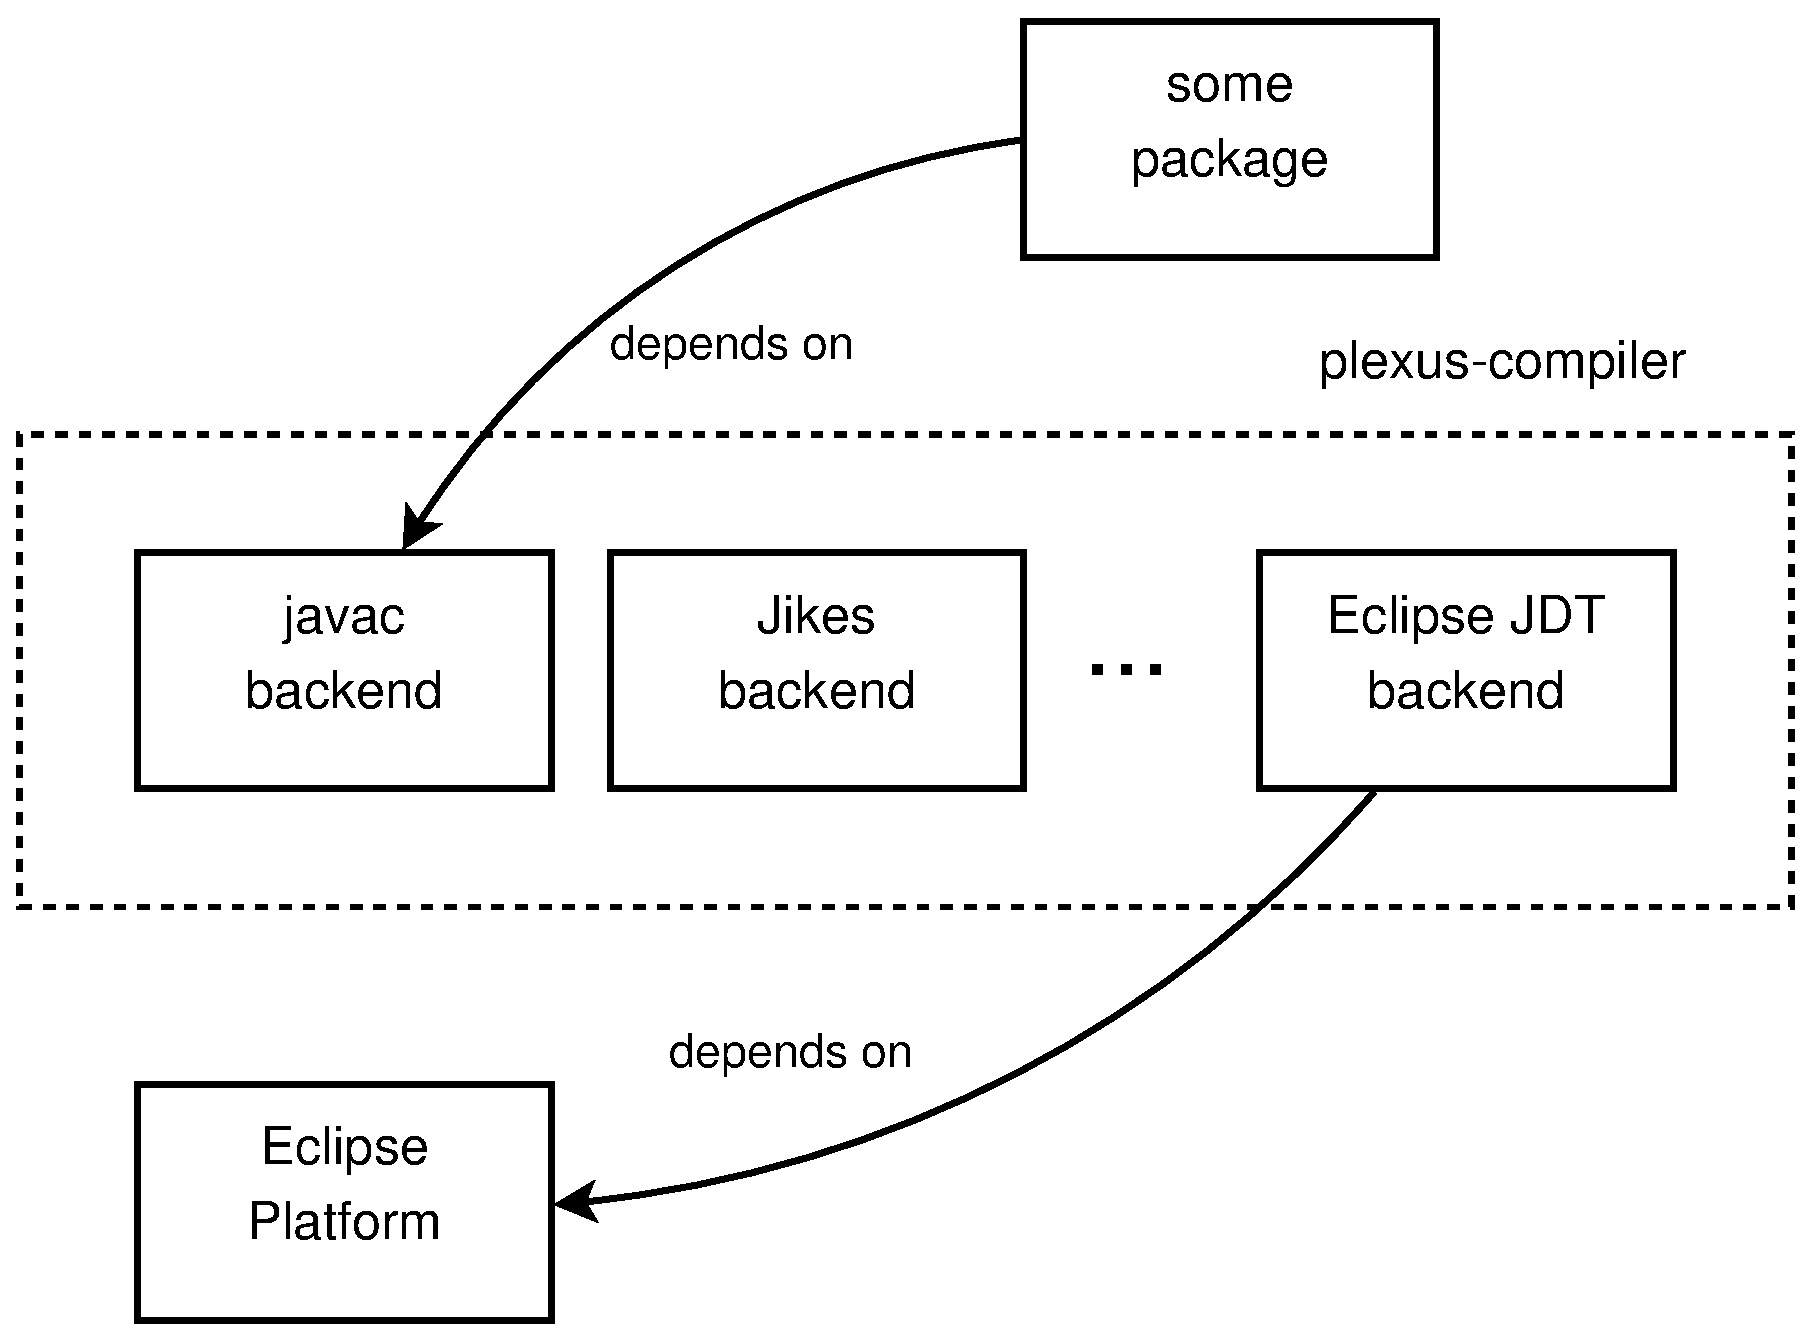
\includegraphics[scale=0.3]{plexus-compiler.eps}
  \end{center}
\end{frame}

\begin{frame}
  \frametitle{A tool is needed}
  \begin{itemize}
    \item Simple usage
    \item Powerfull
    \item Convention over configuration
  \end{itemize}
\end{frame}

\begin{frame}
  \frametitle{Structure of XMvn}
  \begin{itemize}
    \item Portable part
    \begin{itemize}
      \item pure Java
      \item integration with Maven
      \item highly configurable
      \item uses unmodified Maven
    \end{itemize}
    \item Distribution-specific part
    \begin{itemize}
      \item macros and shell scripts
      \item integration with package manager
      \item follows distribution standards
      \item automatic dependency generation
    \end{itemize}
  \end{itemize}
\end{frame}


\begin{frame}[fragile]
  \frametitle{Preparation for the build}
  \begin{block}{Patching POM files}
    \scriptsize
\begin{verbatim}
%pom_add_dep org.apache.commons:commons-io
%pom_disable_module submod-foo
\end{verbatim}
  \end{block}
  \begin{block}{Launching build}
    \scriptsize
\begin{verbatim}
%mvn_file : %{name}
%mvn_build
\end{verbatim}
  \end{block}
\end{frame}


\begin{frame}
  \frametitle{During build}
  \begin{itemize}
    \item Create build plan
    \item Read packgae metadata
    \item Call Maven to build the package
    \begin{itemize}
      \item compile sources
      \item run tests
      \item generate javadocs
    \end{itemize}
    \item Generate matadata
  \end{itemize}
\end{frame}


\begin{frame}[fragile]
  \frametitle{After the build}
  \begin{block}{Installation}
    \scriptsize
\begin{verbatim}
%mvn_install
\end{verbatim}
  \end{block}
  \begin{block}{Enumerating files}
    \scriptsize
\begin{verbatim}
%files -f .mfiles
%files javadoc -f .mfiles-javadoc
\end{verbatim}
  \end{block}
\end{frame}


\begin{frame}[fragile]
  \begin{block}{Example spec file (part 1)}
    \scriptsize
\begin{verbatim}
Name:           maven-shared-incremental
Version:        1.0
Release:        1%{?dist}
Summary:        Maven Incremental Build support utilities
License:        ASL 2.0
Group:          Development/Libraries
URL:            http://maven.apache.org/shared/maven-shared-incremental/
Source0:        http://repo1.maven.org/maven2/org/apache/maven/[...]
BuildArch:      noarch

BuildRequires:  maven-local
BuildRequires:  plexus-component-annotations
BuildRequires:  plexus-component-api

%description
Various utility classes and plexus components for supporting
incremental build functionality in maven plugins.

%package javadoc
Summary:        API documentation for %{name}
Group:          Documentation

%description javadoc
This package provides %{summary}.
\end{verbatim}
  \end{block}
\end{frame}


\begin{frame}[fragile]
  \begin{block}{Example spec file (part 2)}
    \scriptsize
\begin{verbatim}
%prep
%setup -q

%build
%mvn_build

%install
%mvn_install

%files -f .mfiles
%doc LICENSE NOTICE
%dir %{_javadir}/%{name}

%files javadoc -f .mfiles-javadoc
%doc LICENSE NOTICE

%changelog
* Wed Jan 23 2013 Mikolaj Izdebski <mizdebsk@redhat.com> - 1.0-1
- Initial packaging





\end{verbatim}
  \end{block}
\end{frame}

\begin{frame}
  \frametitle{Advantages}
  \begin{itemize}
    \item Simpler, more readable packages
    \item Easier and faster packaging and updates
    \item Better quality packages
    \item Reduced metadata redundancy
    \item No modifications to Maven
    \item Changes in guidelines are easier to introduce
  \end{itemize}
\end{frame}

\begin{frame}[fragile]
  \frametitle{Easier Maven maintenance}
  \begin{block}{Maven diff}
    \scriptsize
\begin{verbatim}
 0001-Add-plugin-api-deps.patch                |  28 --
 0001-Customize-compiler-plugin.patch          | 104 ------
 0002-Use-custom-resolver.patch                | 224 -------------
 0003-Use-utf-8-source-encoding.patch          |  24 --
 ...-scope-skipping-with-maven.test.skip.patch | 160 ---------
 ...ompiler-plugin-default-to-source-1.5.patch |  33 --
 JavadirWorkspaceReader.java                   | 198 -----------
 MavenJPackageDepmap.java                      | 313 ------------------
 maven-empty-dep.jar                           | Bin 341 -> 0 bytes
 maven-empty-dep.pom                           |   9 -
 maven-script-local                            |  47 ---
 maven-script-rpmbuild                         |  93 ------
 maven.spec                                    | 269 +++------------
 repo-metadata.tar.xz                          | Bin 3028 -> 0 bytes
 14 files changed, 37 insertions(+), 1465 deletions(-)
\end{verbatim}
  \end{block}
\end{frame}


\begin{frame}[fragile]
  \frametitle{Build description of maven-surefire in F-12}
  \scriptsize
  \begin{verbatim}
%if %{with_maven}
    export MAVEN_REPO_LOCAL=$(pwd)/.m2/repository
    mkdir -p $MAVEN_REPO_LOCAL
    cat %{SOURCE4}
    mvn-jpp -e -Dmaven.repo.local=$MAVEN_REPO_LOCAL \
        -Dmaven2.jpp.depmap.file=%{SOURCE4} \
        -Dmaven.test.skip=true install
    for dir in maven-surefire-plugin maven-surefire-report-plugin \
               surefire-api surefire-booter surefire-providers/surefire-junit; do
        (cd $dir
         mvn-jpp -Dmaven.repo.local=$MAVEN_REPO_LOCAL \
                 -Dmaven2.jpp.depmap.file=%{SOURCE4} \
                 javadoc:javadoc
        )
    done
%else
    mkdir -p lib
    build-jar-repository -s -p lib classworlds junit plexus/utils
    ant -Dmaven.mode.offline=true
    cp -p target/*jar ../lib/$project.jar
%endif
  \end{verbatim}
  \note{Note!}
\end{frame}

\begin{frame}[fragile]
  \frametitle{Build description of maven-surefire in F-15}
  \scriptsize
  \begin{verbatim}
# tests turned off because they need jmock
mvn-rpmbuild -e \
        -Dmaven.local.depmap.file=%{SOURCE1} \
        -Dmaven.test.skip=true \
        install javadoc:aggregate
  \end{verbatim}
  \note{Note!}
\end{frame}

\begin{frame}[fragile]
  \frametitle{Build description of maven-surefire in F-19}
  \scriptsize
  \begin{verbatim}
%mvn_build -f
  \end{verbatim}
  \note{Note!}
\end{frame}


\begin{frame}[fragile]
  \frametitle{Simplified package}
  \begin{block}{maven-surefire diff between F-12 and F-18}
    \scriptsize
\begin{verbatim}
 .cvsignore                           |   3 -
 .gitignore                           |  14 +
 Makefile                             |  21 --
 maven-surefire-2.3-junit4-pom.patch  |  11 -
 maven-surefire-booter-build.xml      |  64 -----
 maven-surefire-build.xml             |  90 ------
 maven-surefire-buildonlyjunit3.patch |  13 -
 maven-surefire-buildskiptestng.patch |  12 -
 maven-surefire-jpp-depmap.xml        |  23 --
 maven-surefire-plexus12.patch        |  20 --
 maven-surefire.spec                  | 399 +++++++--------------------
 sources                              |   3 +-
 12 files changed, 117 insertions(+), 556 deletions(-)
\end{verbatim}
  \end{block}
\end{frame}

\begin{frame}
  \frametitle{Disadvantages}
  \begin{itemize}
    \item Less control
    \item Harder to debug
    \item Incompatibility with older systems
    \item Bleeding edge
  \end{itemize}
\end{frame}

\begin{frame}
  \frametitle{Summary}
  \begin{itemize}
    \item Improved packaging
    \item Full solution
    \item Backwards-compatible
    \item Smooth transition
  \end{itemize}
\end{frame}


\begin{frame}
  \frametitle{Future}
  \begin{itemize}
    \item Automated package generation
    \item Debugging tools
    \item Graphical tooling
    \item Support for more types of artifacts
    \item Integration with Eclipse
    \item Adoption by different distributions?
  \end{itemize}
\end{frame}



\mode<presentation> {
  \Rhbg{\frame{\theend}}
}

\end{document}
